\textbf{Use Cases 3-8}\\
Disse Use Cases beskriver følgende funktionalitet:
\begin{itemize}
	\item Opret produkt
	\item Rediger produkt
	\item Slet produkt
	\item Opret kategori
	\item Rediger kategori
	\item Slet kategori
\end{itemize}
Funktionaliteten til disse Use Cases ligner hinanden. Når gls{SB} har udført de nødvendige handlinger i \gls{AS}ets grafiske brugerflade og trykker på knappen til at godkende handlingen, så bliver der sendt data til \gls{CS} og efterfølgende modtaget data fra \gls{CS}.

Når \gls{SB} har modificeret et produkt eller en kategori i \gls{AS}, så vil følgende handlinger blive udført i systemet:
\begin{itemize}
	\item \gls{AS} opretter et kommando objekt af den rette type, med informationerne for handlingen.
	\item \gls{AS} bruger \gls{SL} til at konvertere kommando objektet til en XML streng.
	\item XML strengen sendes til \gls{CS}.
	\item \gls{CS} modtager strengen og konverterer den tilbage til den oprindelige kommando, igen ved hjælp af \gls{SL}.
	\item \gls{CS} udfører de nødvendige handlinger på \gls{DB}.
	\item \gls{CS} opretter et kommando objekt med det rette svar (f.eks. ProductCreated efter den har oprettet et produkt).
	\item \gls{CS} konverterer kommandoen til en XML streng ved hjælp af \gls{SL}.
	\item \gls{CS} sender XML strengen til alle de klienter der er forbundet til \gls{CS}.
\end{itemize}

Funktionaliteten for Use Casene er beskrevet med et sekvensdiagram, som vises på figur \ref{fig:uc38sq}.

\begin{figure}[H]
    \centering
    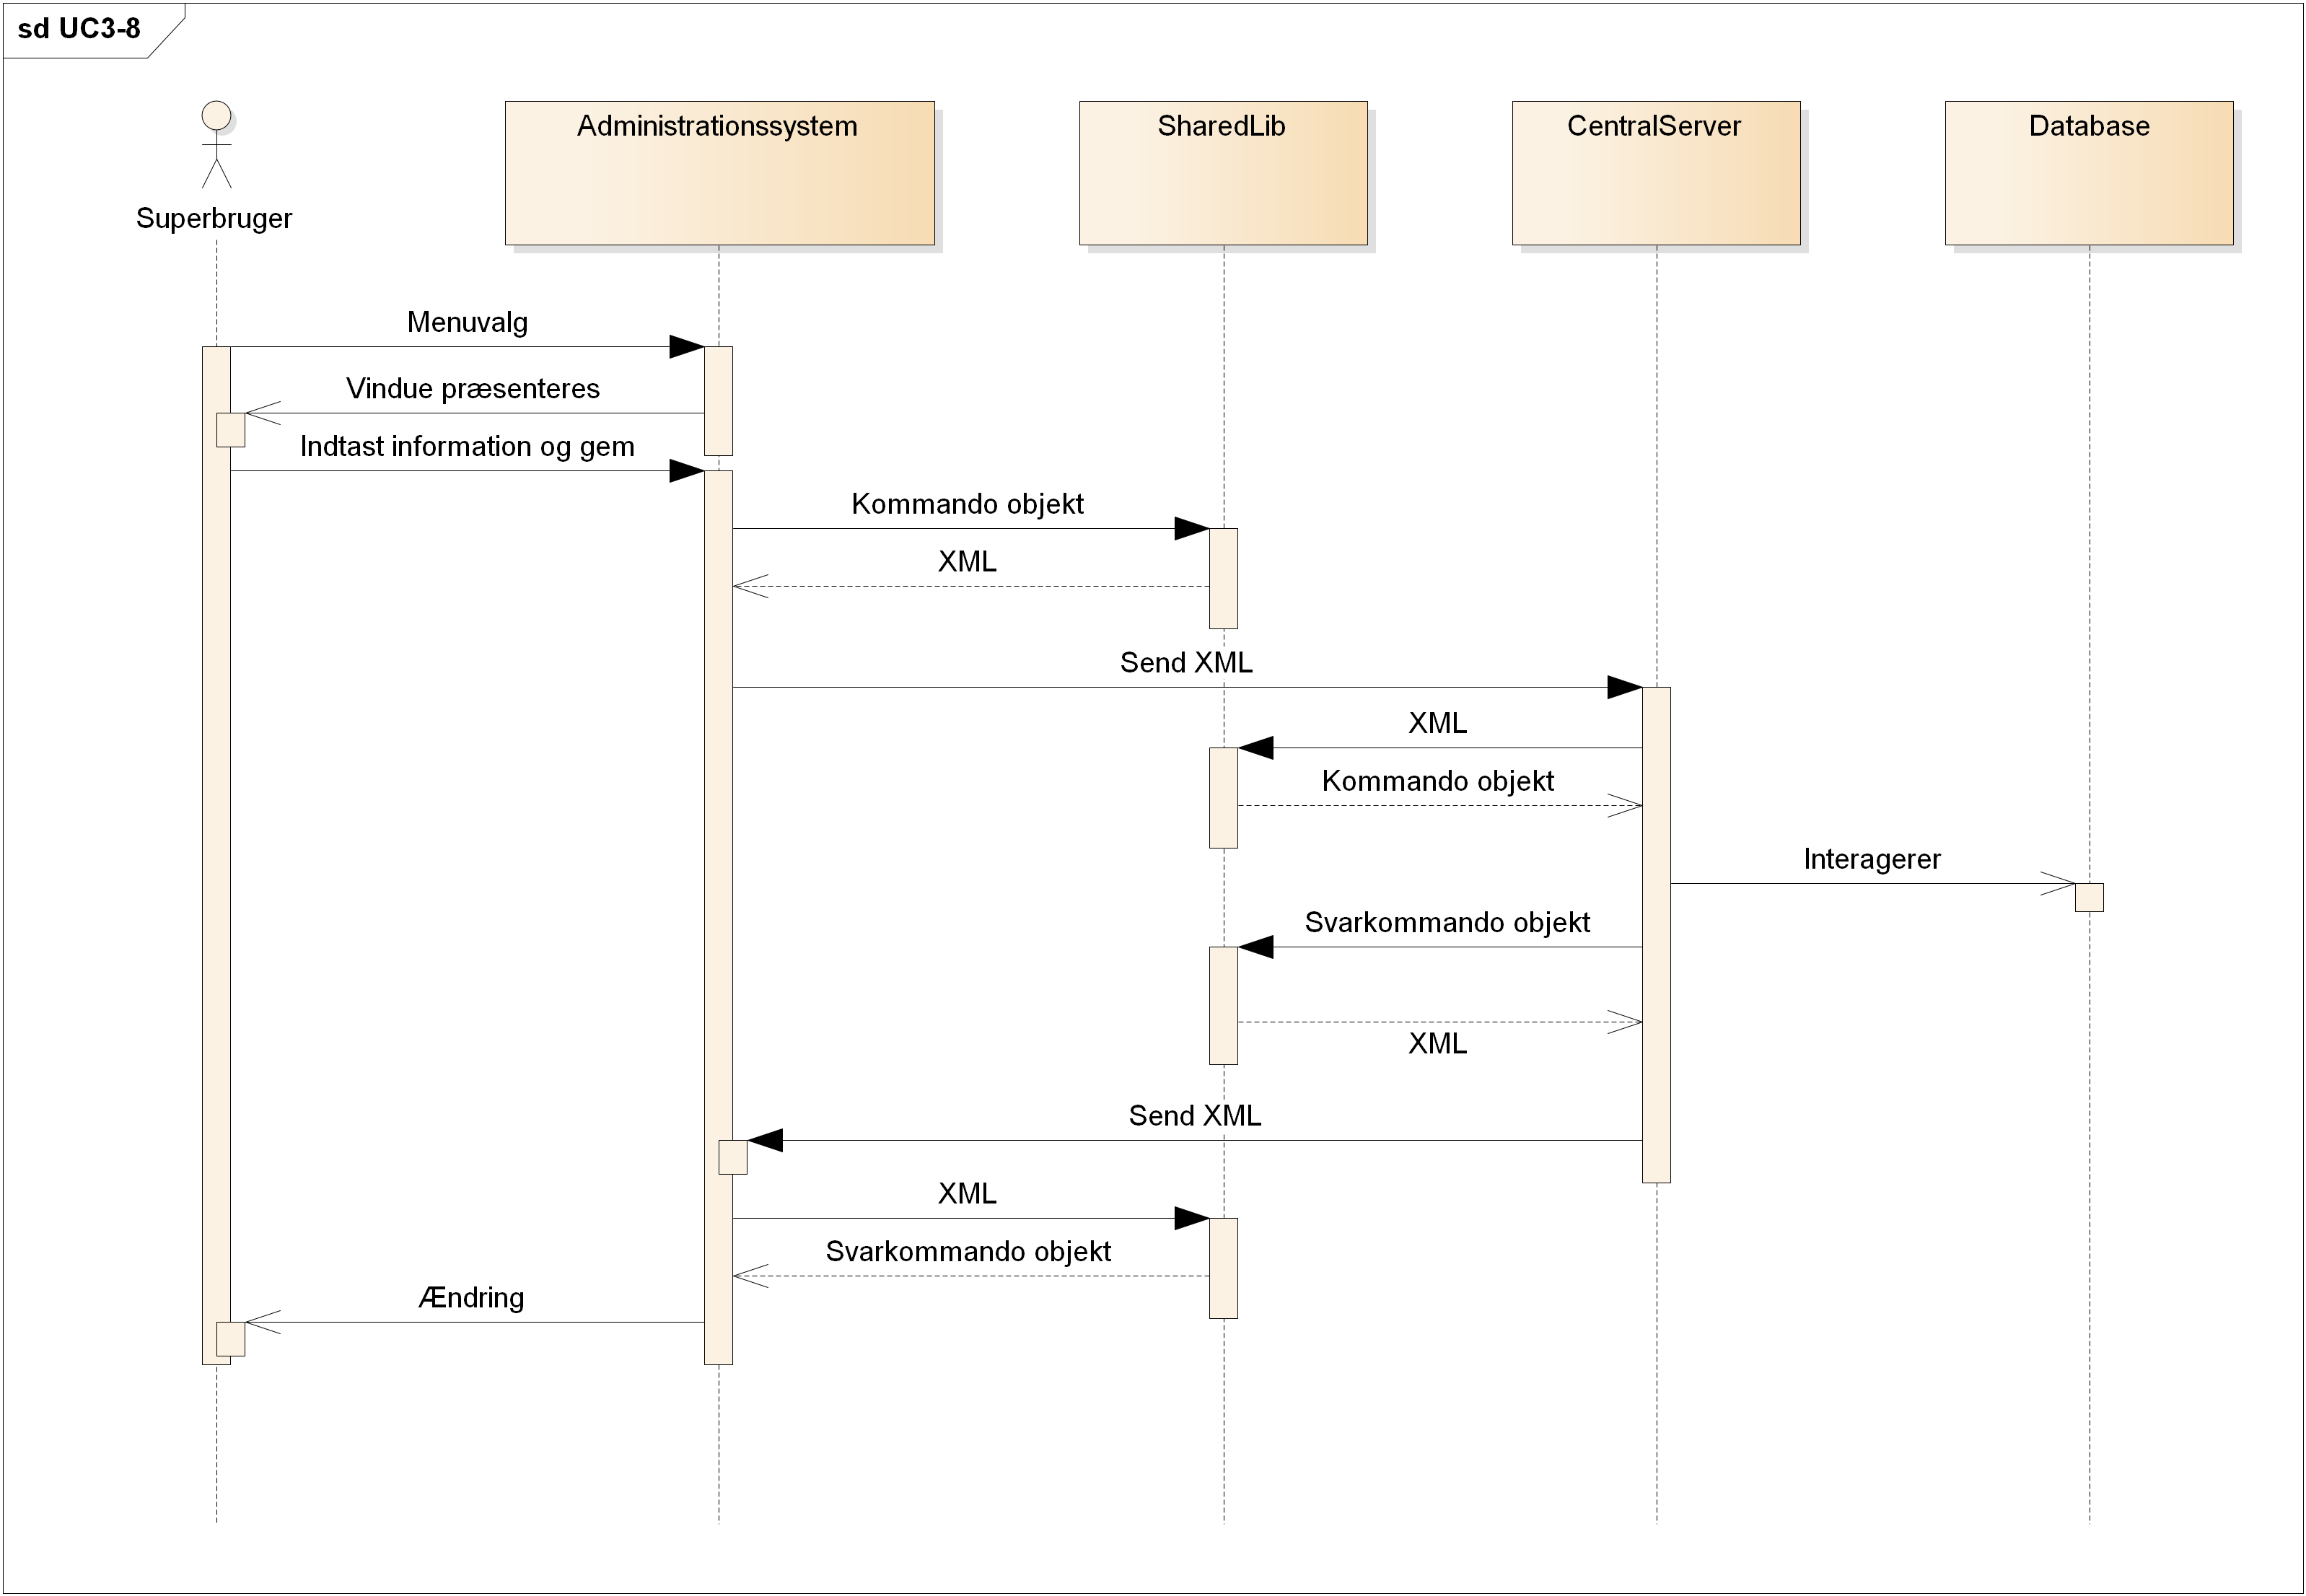
\includegraphics[width=0.8\textwidth]{Systemarkitektur/LogiskView/Realiseringer/Images/UC38.png}
    \caption{Sekvensdiagram for realisering af Use Cases 3 til 8.}
    \label{fig:uc38sq}
\end{figure}

Når CentralServer svarer, er der på sekvensdiagrammet (figur \ref{fig:uc38sq}) afbilledet, at den blot svarer til Administrationssystemet. I realiteten broadcaster den svaret til alle klienter der er forbundet. Dette er dog ikke vigtigt for forståelsen af kommunikationen i disse Use Cases.